\section{Descripción estructural \label{sec:s1}}

\begin{center}
	\begin{minipage}{12cm}
		\begin{tcolorbox}[title=Actividad 1]
			Capturar el código para describir en forma estructural el multiplexor en el lenguaje de su elección. Instanciar el módulo o componente que se encuentre en el mismo archivo. Simular el multiplexor.
		\end{tcolorbox}	
	\end{minipage}
\end{center}

La visualización RTL del producto punto de dos vectores, empleando For-Loop en VHDL, se muestra en la \autoref{fig:for_loop1_vhdl_rtl}. Como se observa, la implementación se realiza utilizando 4 instancias de sumadores de 16 bits, 4 instancias de multiplicadores de 8 bits, un decodificador, algunas compuertas lógicas AND para apoyar al decodificador y 64 latches que se utilizan para almacenar cada bit de cada dato ubicado en las localidades de Vector1 y Vector2. Las simulaciones se visualizan en la \autoref{fig:for_loop1_vhdl_wavebi} en base binaria y en la \autoref{fig:for_loop1_vhdl_wavede} en base decimal, en donde se muestra que la operación producto punto de ambos vectores es correcta.

En los Anexos se localiza la descripción en VHDL de este modulo de producto punto. La implementación se hace declarando las librerías y la entidad, junto con las señales de entradas y salida correspondientes. En la zona declarativa se declara un arreglo de 4 localidades de 8 bits de tamaño y después se crean 2 arreglos de este tipo, denominados Vector1 y Vector2 y se inicializan los valores de cada localidad. Al entrar a la declaración de arquitectura se generan dos lista sensibles:

\begin{itemize}
	\item La primera, evalúa si esta habilitada la señal WR, en caso de ser así, se escriben los datos de entrada en la dirección indicada por la señal DIR.
	\item La segunda, genera el cálculo del producto punto, usando una variable de apoyo (Var) para hacer la suma de los productos y otra variable (i) para iterar las operaciones. Cabe señalar que la primer variable mencionada se inicializa en 0, para realizar la suma aritmética de manera correcta. Al final de las iteraciones, se asigna el valor de la variable a la señal de salida.
\end{itemize}

\begin{figure}[ht]
	\centering
	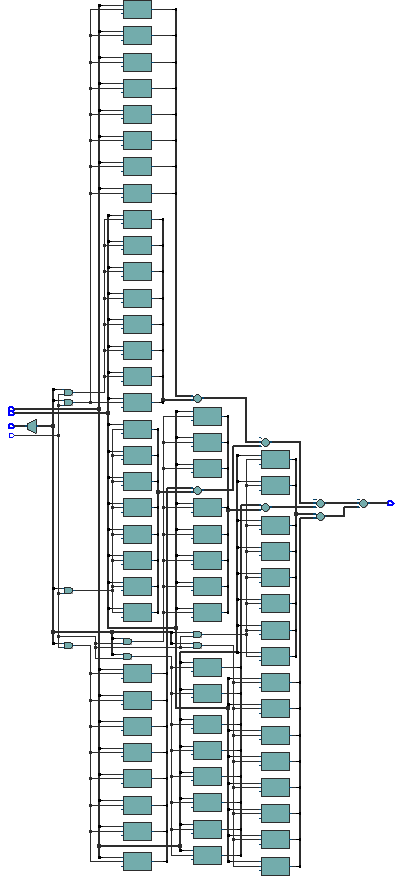
\includegraphics[scale=0.9]{For_Loop1_VHDL_RTL.png}
	\caption{Diagrama RTL del producto punto de dos vectores implementado en VHDL. \label{fig:for_loop1_vhdl_rtl}}
\end{figure}

\begin{figure}[ht]
	\centering
	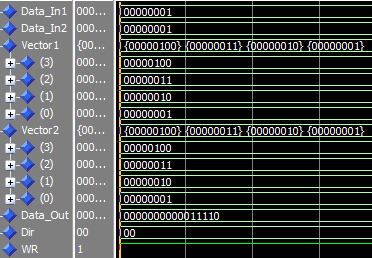
\includegraphics[scale=1.4]{For_Loop1_VHDL_WaveBi.png}
	\caption{Simulación del producto punto de dos vectores en VHDL con el visor de formas de onda de ModelSim (base binaria). \label{fig:for_loop1_vhdl_wavebi}}
\end{figure}

\begin{figure}[ht]
	\centering
	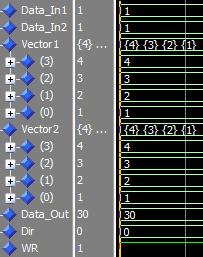
\includegraphics[scale=1.4]{For_Loop1_VHDL_WaveDe.png}
	\caption{Simulación del producto punto de dos vectores en VHDL con el visor de formas de onda de ModelSim (base decimal). \label{fig:for_loop1_vhdl_wavede}}
\end{figure}